\documentclass[12pt]{article}

\usepackage[left=1cm, right=1cm, top=2cm, bottom=1mm]{geometry}
\usepackage{float}
\usepackage{graphicx}
\usepackage{hyperref}
\usepackage{xcolor}
\usepackage{amsmath}

\title{Technical Assesment - WIND Project} 
\author{Kristoforus Bryant Odang}

\begin{document}
\maketitle


\section{Introduction}
Below are the results for the WIND Project Technical Assesment. The main document is kept at 3 pages, but I include an appendix of all the result. The code implementation of this assesment can be found in \url{https://github.com/kristoforusbryant/cv-technical-assesment-wind}. 

\section{Task 1: Circle Detection}

\subsection{Method Used}
For this task, I use the Circles Hough Transform, after blurring and converting the images to grayscale. The Circles Hough Transform does well on this problem. To optimise computation, I resized the image to 1/16 of its size before applying the transformations.

\subsection{Results}
Note following success cases.

\begin{figure}[H]
\centerline{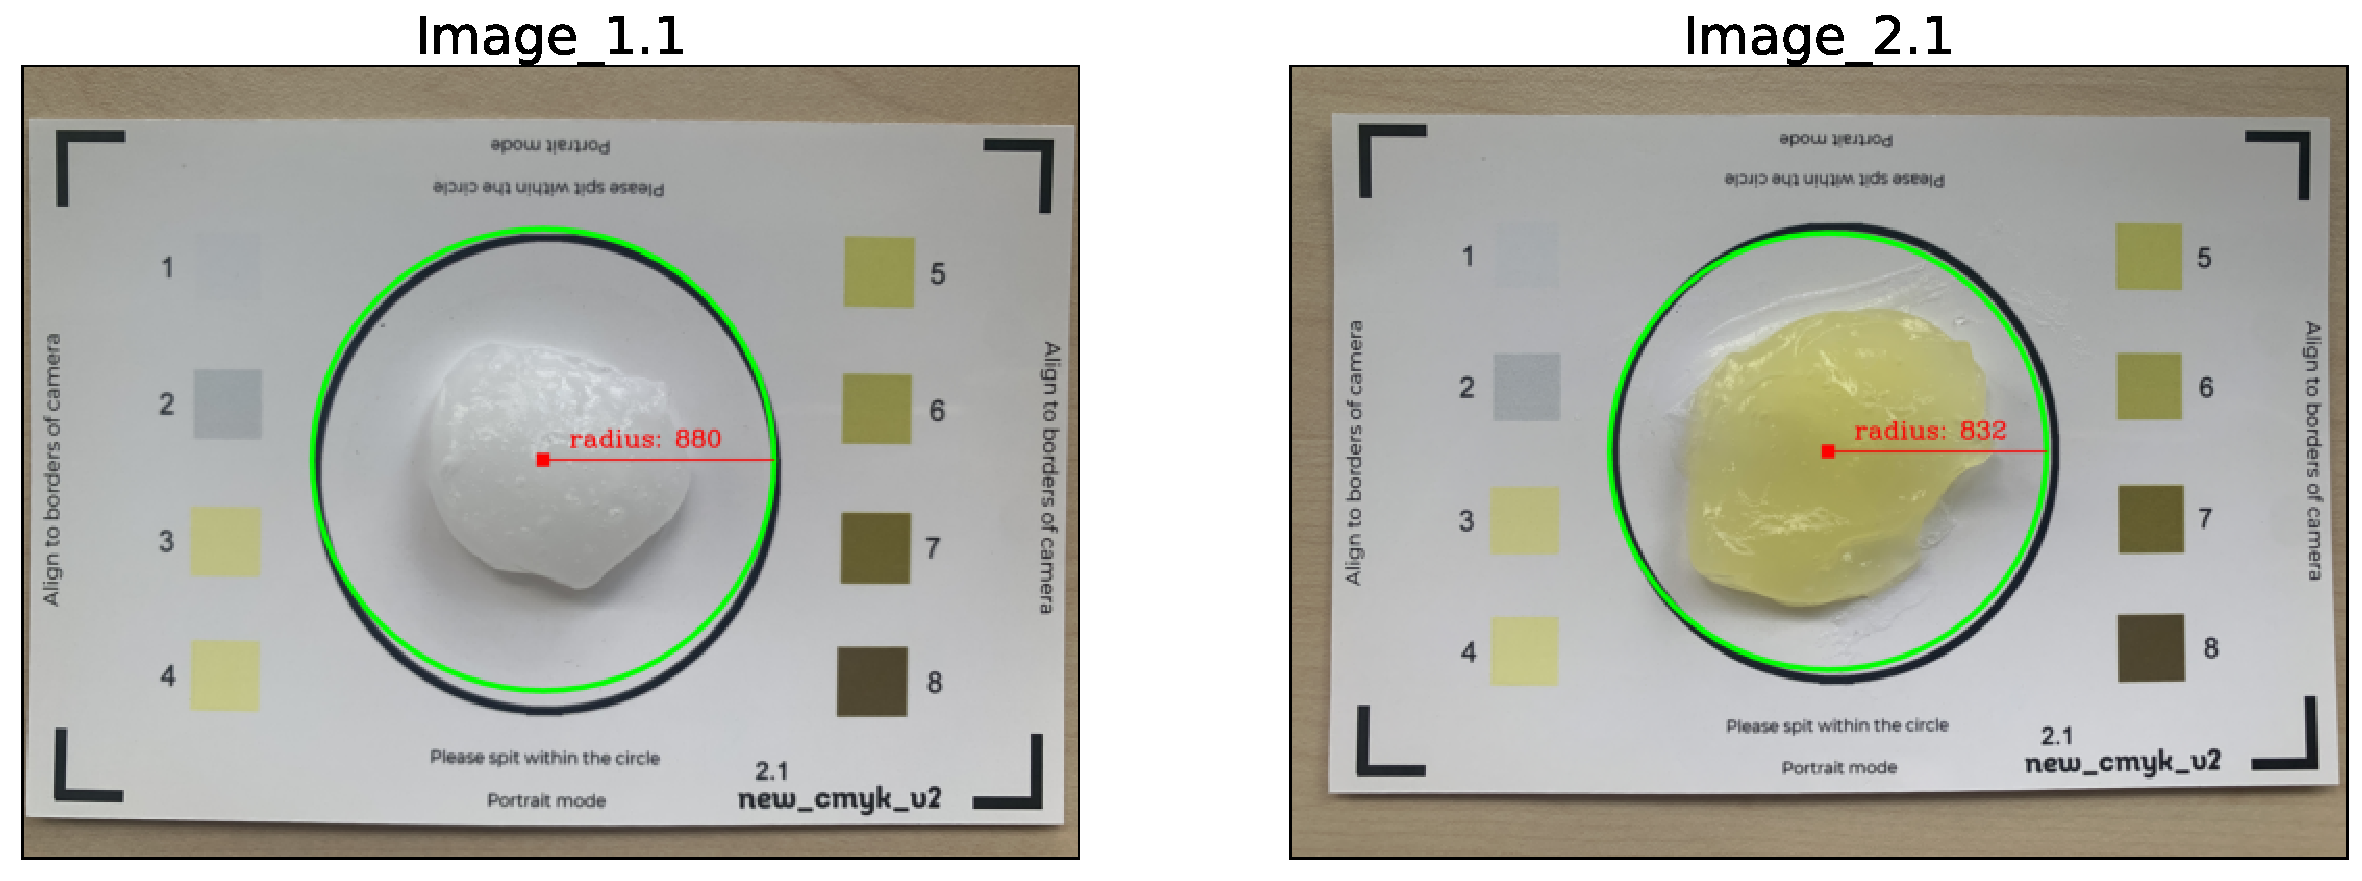
\includegraphics[width=.85\textwidth]{figs/task1-success.pdf}} 
	\caption{Examples of success cases in Task 1.}
	\label{fig: task1-success}
\end{figure}
No serious failure cases detected.

\section{Task 2: Squares Detection}
\subsection{Method Used}
To obtain the boundary around the squares, the method follows three steps. Firstly, noting that the position of the squares remain the same across different images, from a grid (see Fig~\ref{fig: task2-grid}) I slice 8 rectangles, each containing exactly one square. This grid is arbitrarily chosen based on visual inspection of the samples given and thus sensitive to the boundaries of the camera. 

For each of these slices, I split the image into its HSV and RGB channels. From testing on some examples (see Fig~\ref{fig: task2-color}), I notice that for squares 3 - 8, the saturation (S) channel from the HSV decomposition separates the squares from the background most. Whilst, for square 2, the blue (B) channel from the RGB decomposition separates square 2 most from the background. Unfortunately,  square 1 is too similar to the background, hence, like square 2 for this I also used the blue channel for further processing.

After getting the S or G channel depening on the squares, I find the contour and draw a bounding box around that contour. This is what is seen in the results.

\subsection{Results}
The following shows one success case and the most serious failure case from this task.

\begin{figure}[H]
\centerline{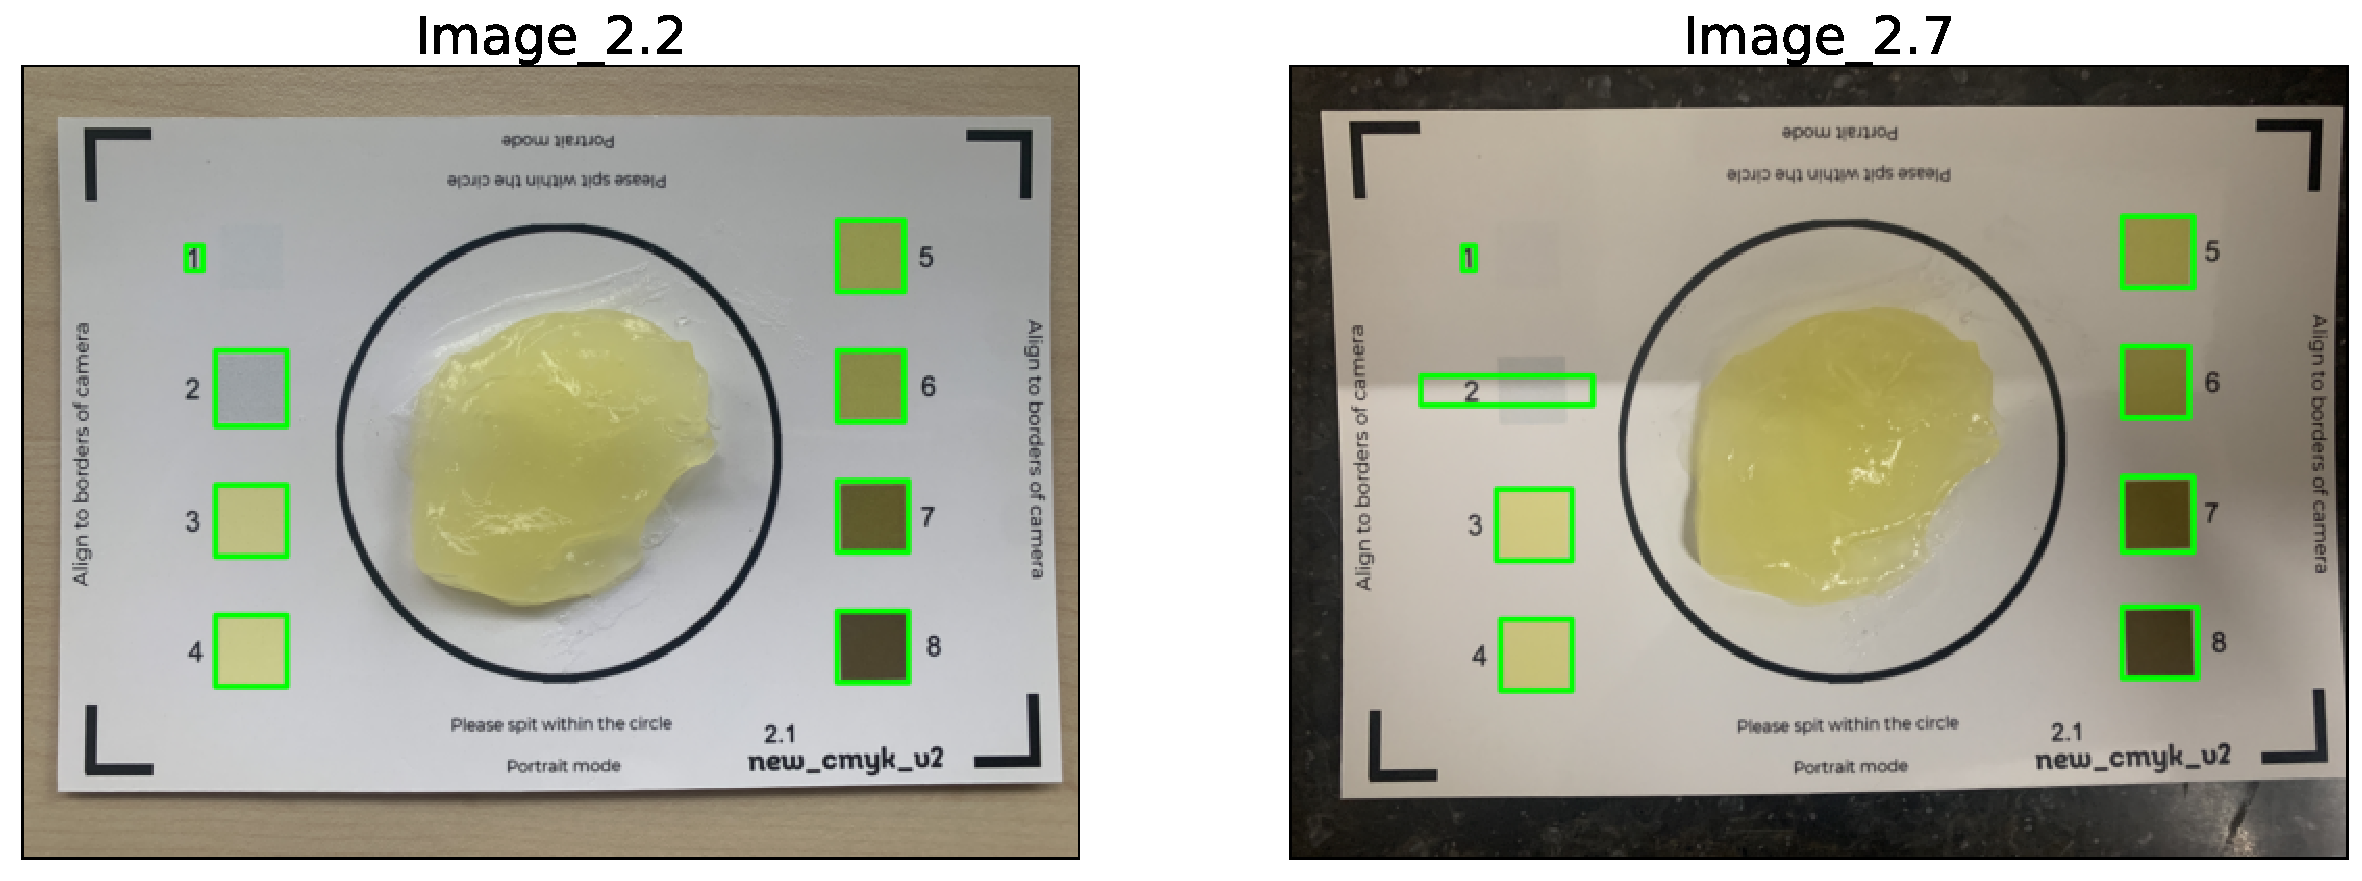
\includegraphics[width=.85\textwidth]{figs/task2-results.pdf}} 
	\caption{One success and one failure case each from Task 2.}
	\label{fig: task2-results}
\end{figure}

Note that there are two serious failures with the implemented algorihtm. Firstly, the algorithm fails on most cases to detect the square labled 1. This is likely due to the lack of sufficient contrast between the colour of square 1 and the colour of thed background. This difference in colours is even difficult to detect with naked eye. Instead of detecting the square, the algorihtm draws a box around the number 1. This is because the number 1 is the largest detected object on the defined grid. This problem is difficult to solve since the image itself does not give enough contrast for the algorithm to detect. A heuristic that can be used is to take the x and y values from the bottom-left corner of square 3 and square 5, respectively, and draw a square with the width and height of one of the reliable square estimates (3 - 8), taking that point at its bottom-left corner. This can be a solution noting that the position of the squares are invariant relative (to one another) across different pictures.

The second serious failure happens when the picture contains a sharp shadow. For example, in Figure~\ref{fig: task2-results}, prediction on square 2 is inaccurate as the algorithm detects the shadow as an edge. This can possibly solved using a shadow removal algorithm.

\section{Task 3 (and Bonus): Sample Boundaries}
\subsection{Method Used}
To obtain the boundary around the sample. Firstly, I apply the canny edge procedure to the grayscale-transformed image. Then using the method in Task 1, remove edges detected on the perimiter or outside the circle. Then, I find the contours of the remaining edges. The outlines seen around the samples are the convex hull of the union of points of every contour.

\subsection{Results}
The following shows one success case and the most serious failure case from this task.
\begin{figure}[H]
\centerline{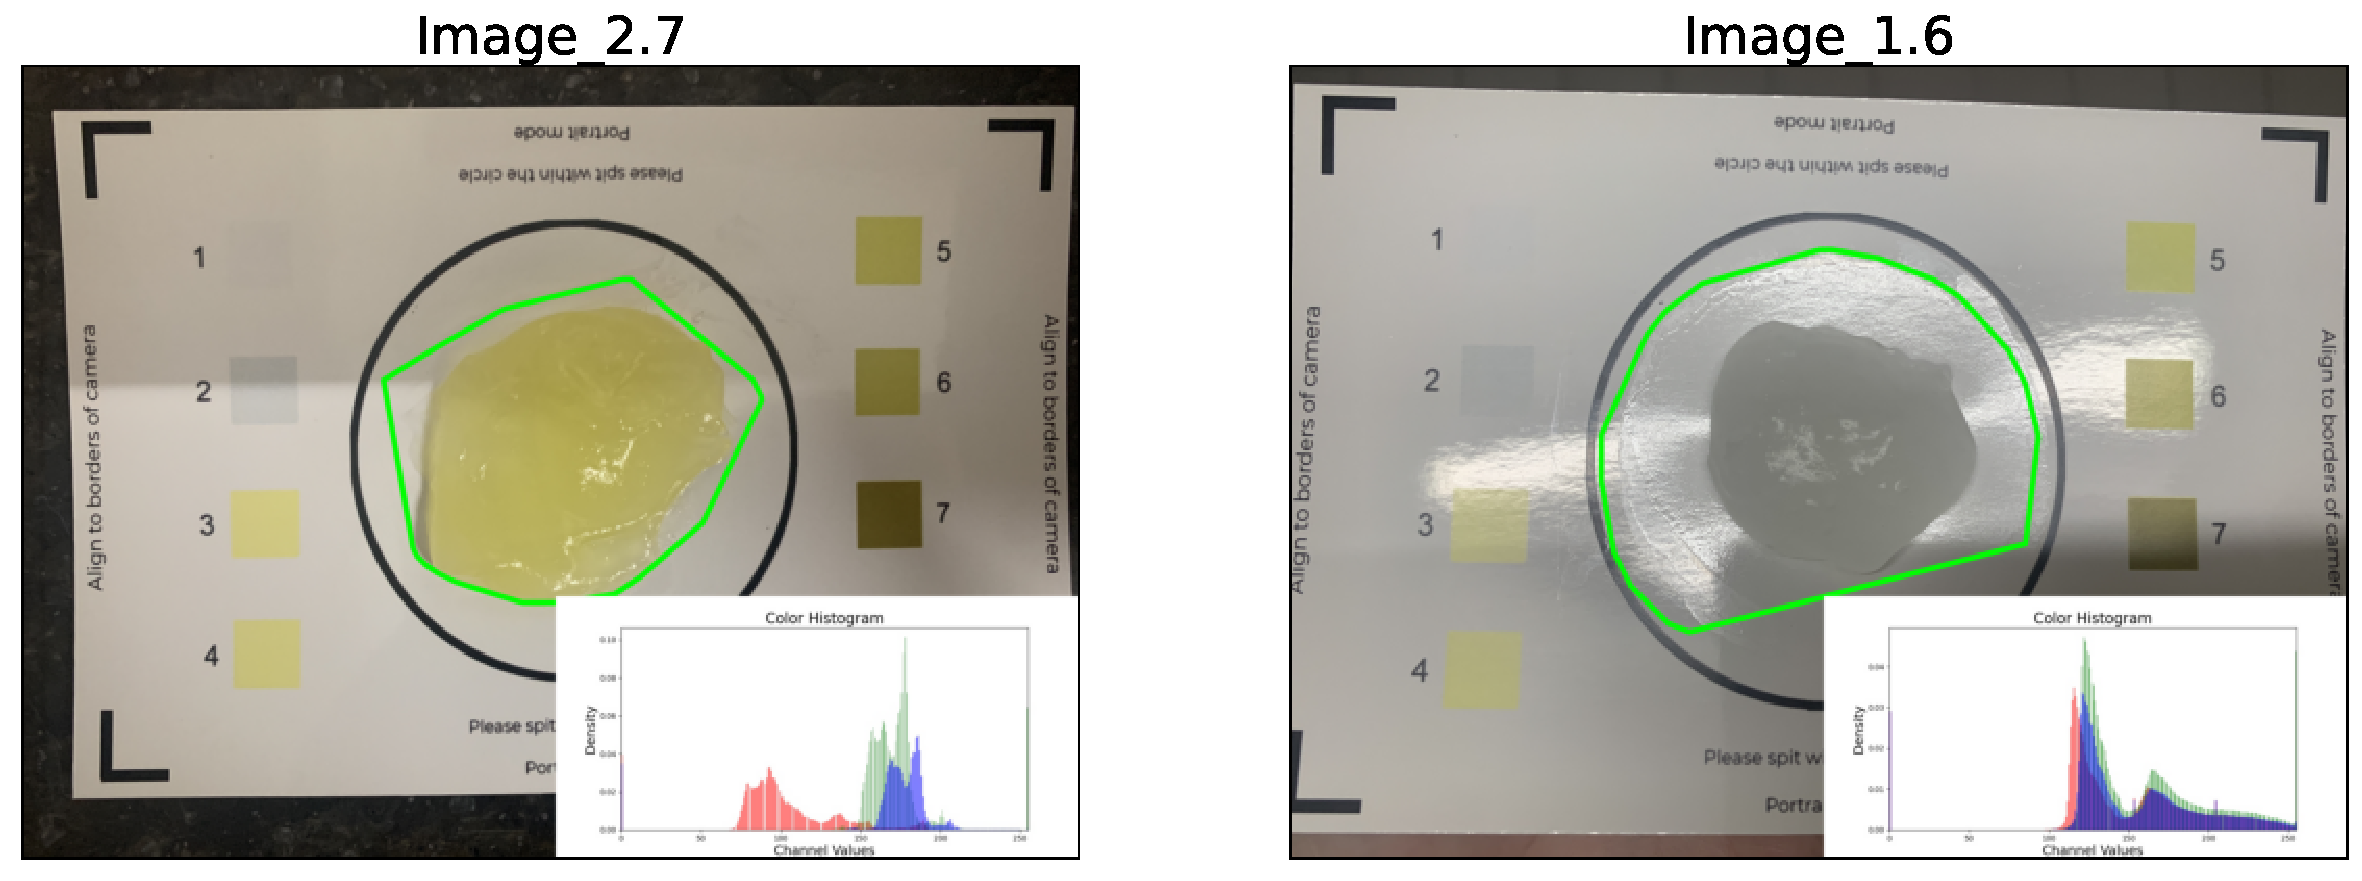
\includegraphics[width=.85\textwidth]{figs/task3-results.pdf}} 
	\caption{One success and one failure case each from Task 3.}
	\label{fig: task3-results}
\end{figure}

As seen in Figure~\ref{fig: task3-results}, the reflection of a light source from the background can prevent the algorithm from detecting the sample. This is because the algorithm detects the reflection as a contour, hence the convex hull includes the edges of the reflection. Being able to remove the reflection is necessary for the algorithm to perform in these cases.

\section{Discussion}
In this document I present the results the tasks given. From the failure cases, I noticed that the shadow and illumination is the primary cause for the failures of my algorithms. Thus, it might be of interest to explore shadow and glare removal methods. Moreover, while the algorihtm in Task 2 does reasonably well for squares 3-8, my algorithm rely being able to find grids that contains one square each. This is currently using a manual threshold, considering the samples given. However, an automated way can be devised to detect these grids, for example by first standardizing the image using methods such as getPerspectiveTransform in openCV.

\newpage
\section{Appendix}

\begin{figure}[h]
    \centerline{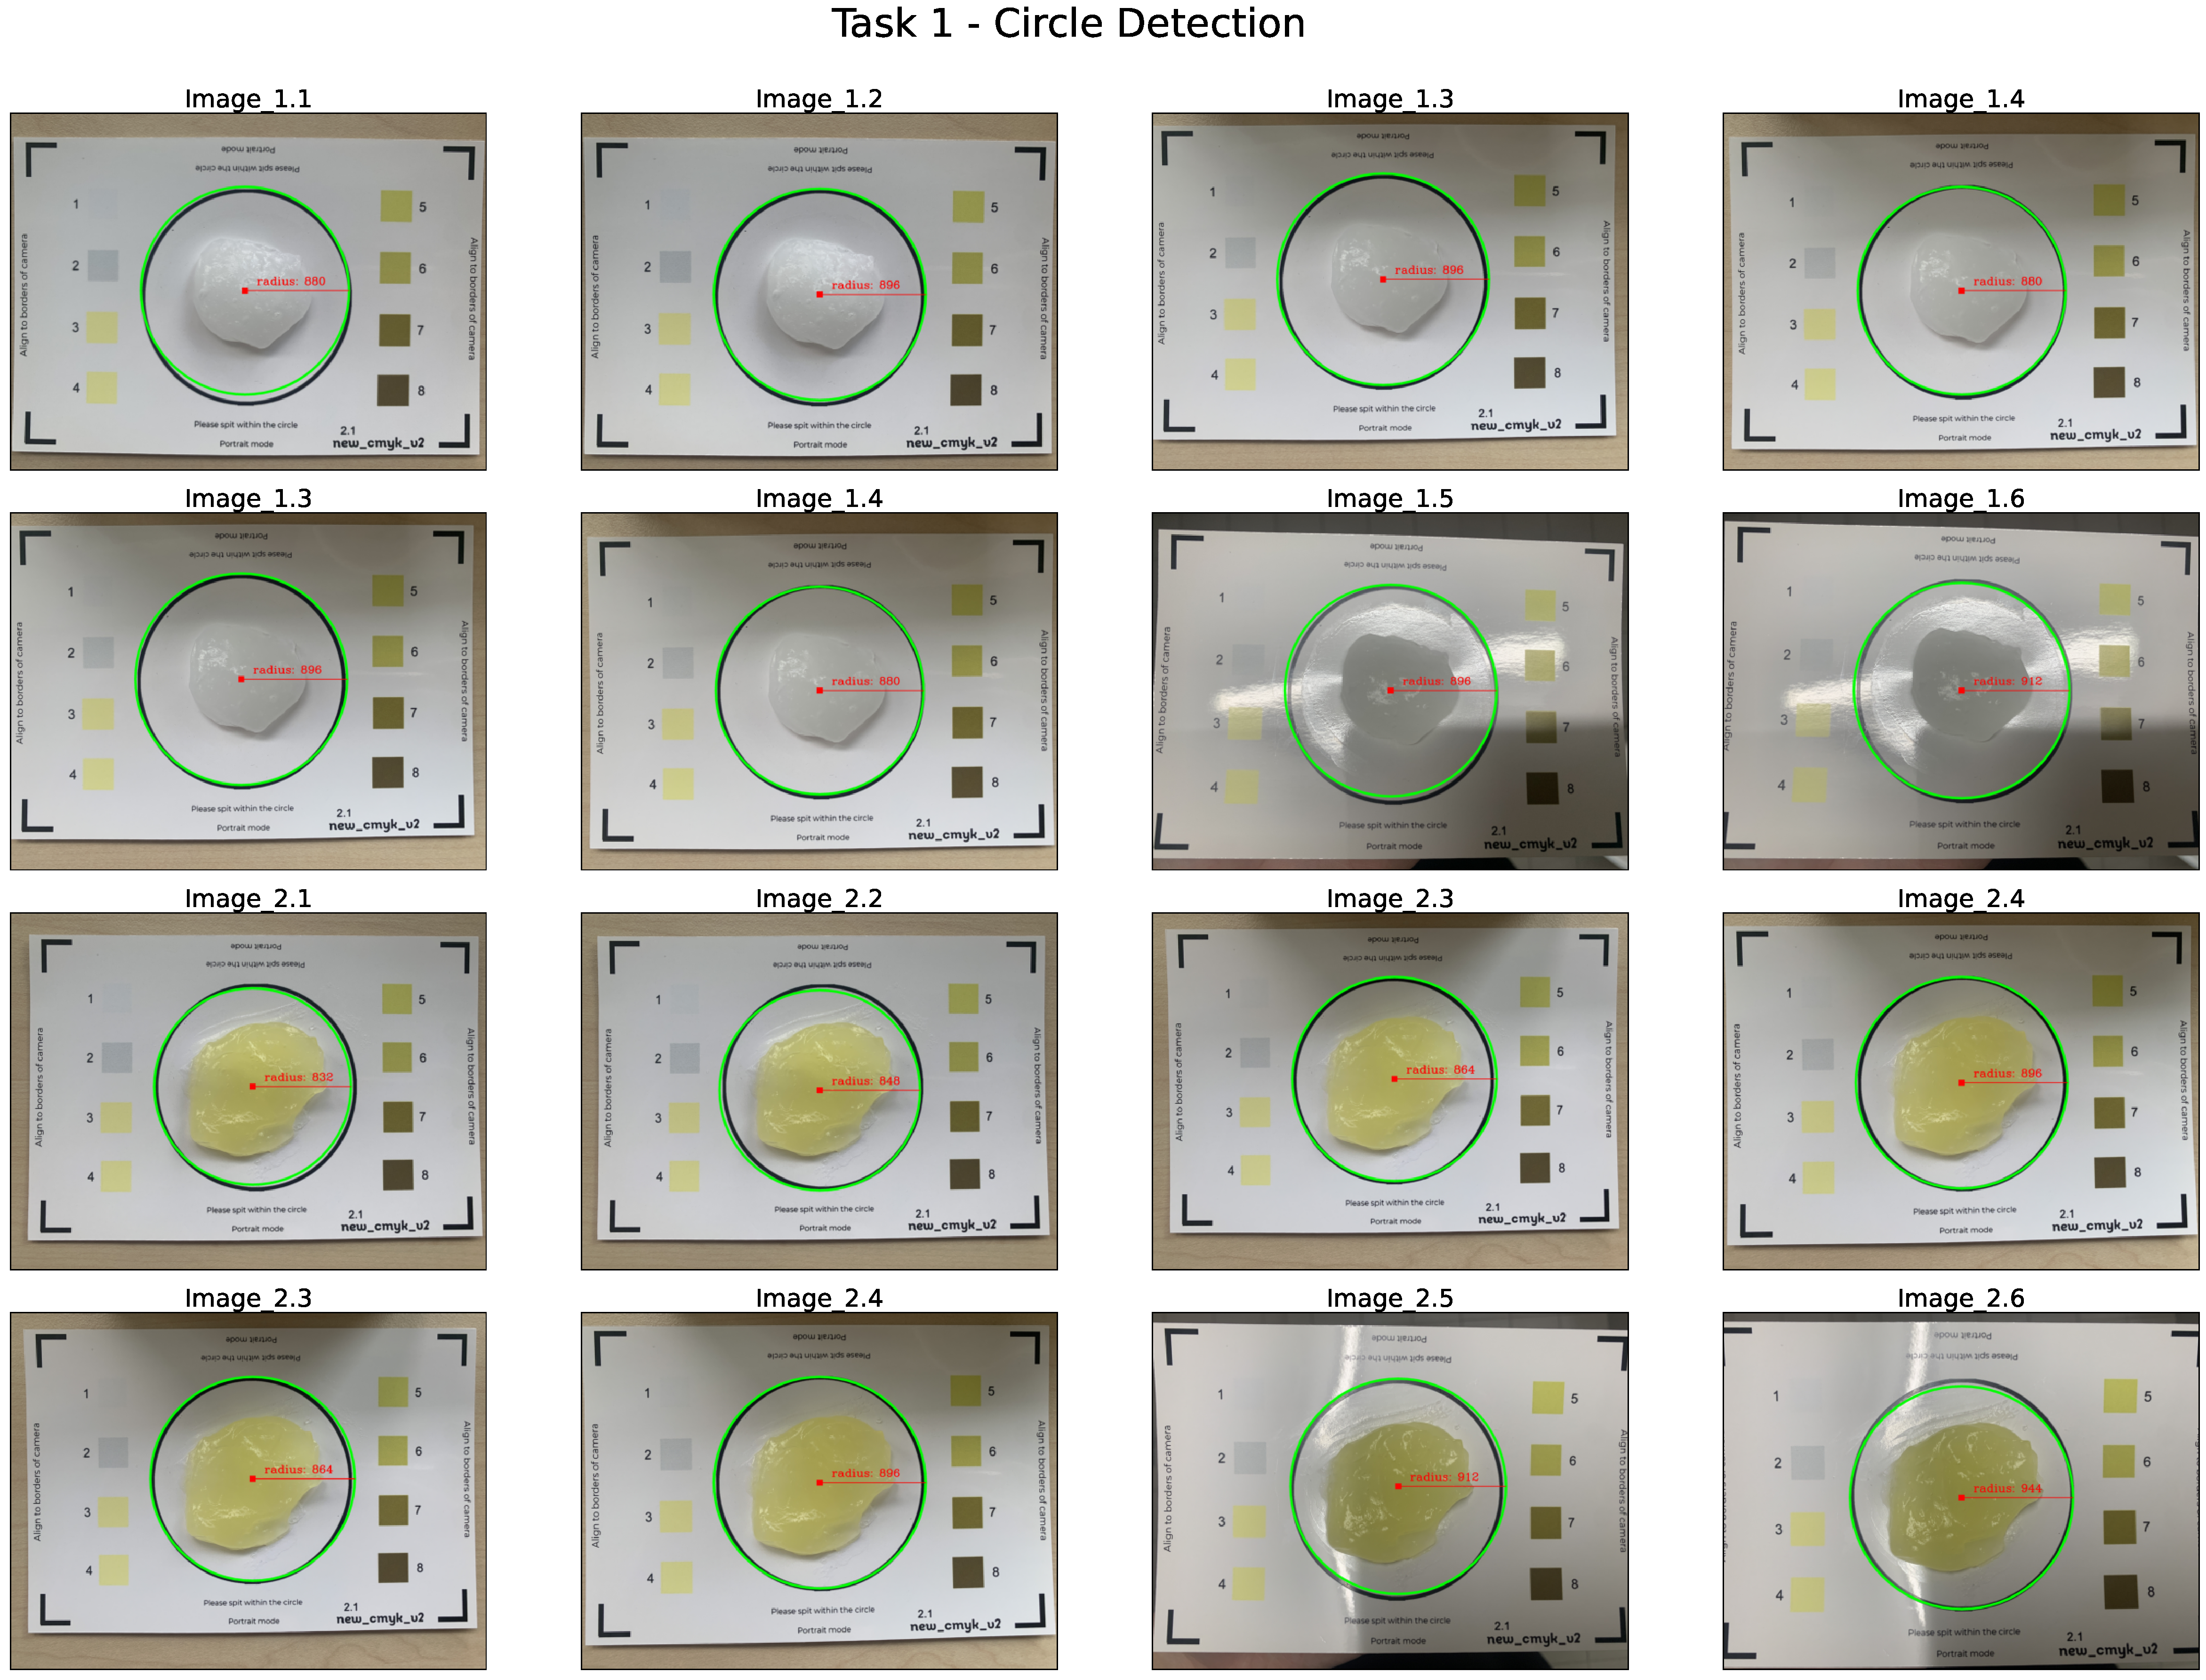
\includegraphics[width=\textwidth]{figs/task1.pdf}} 
	\caption{All results from Task 1.}
	\label{fig: task1-all}
\end{figure}

\newpage

\begin{figure}[h]
    \centerline{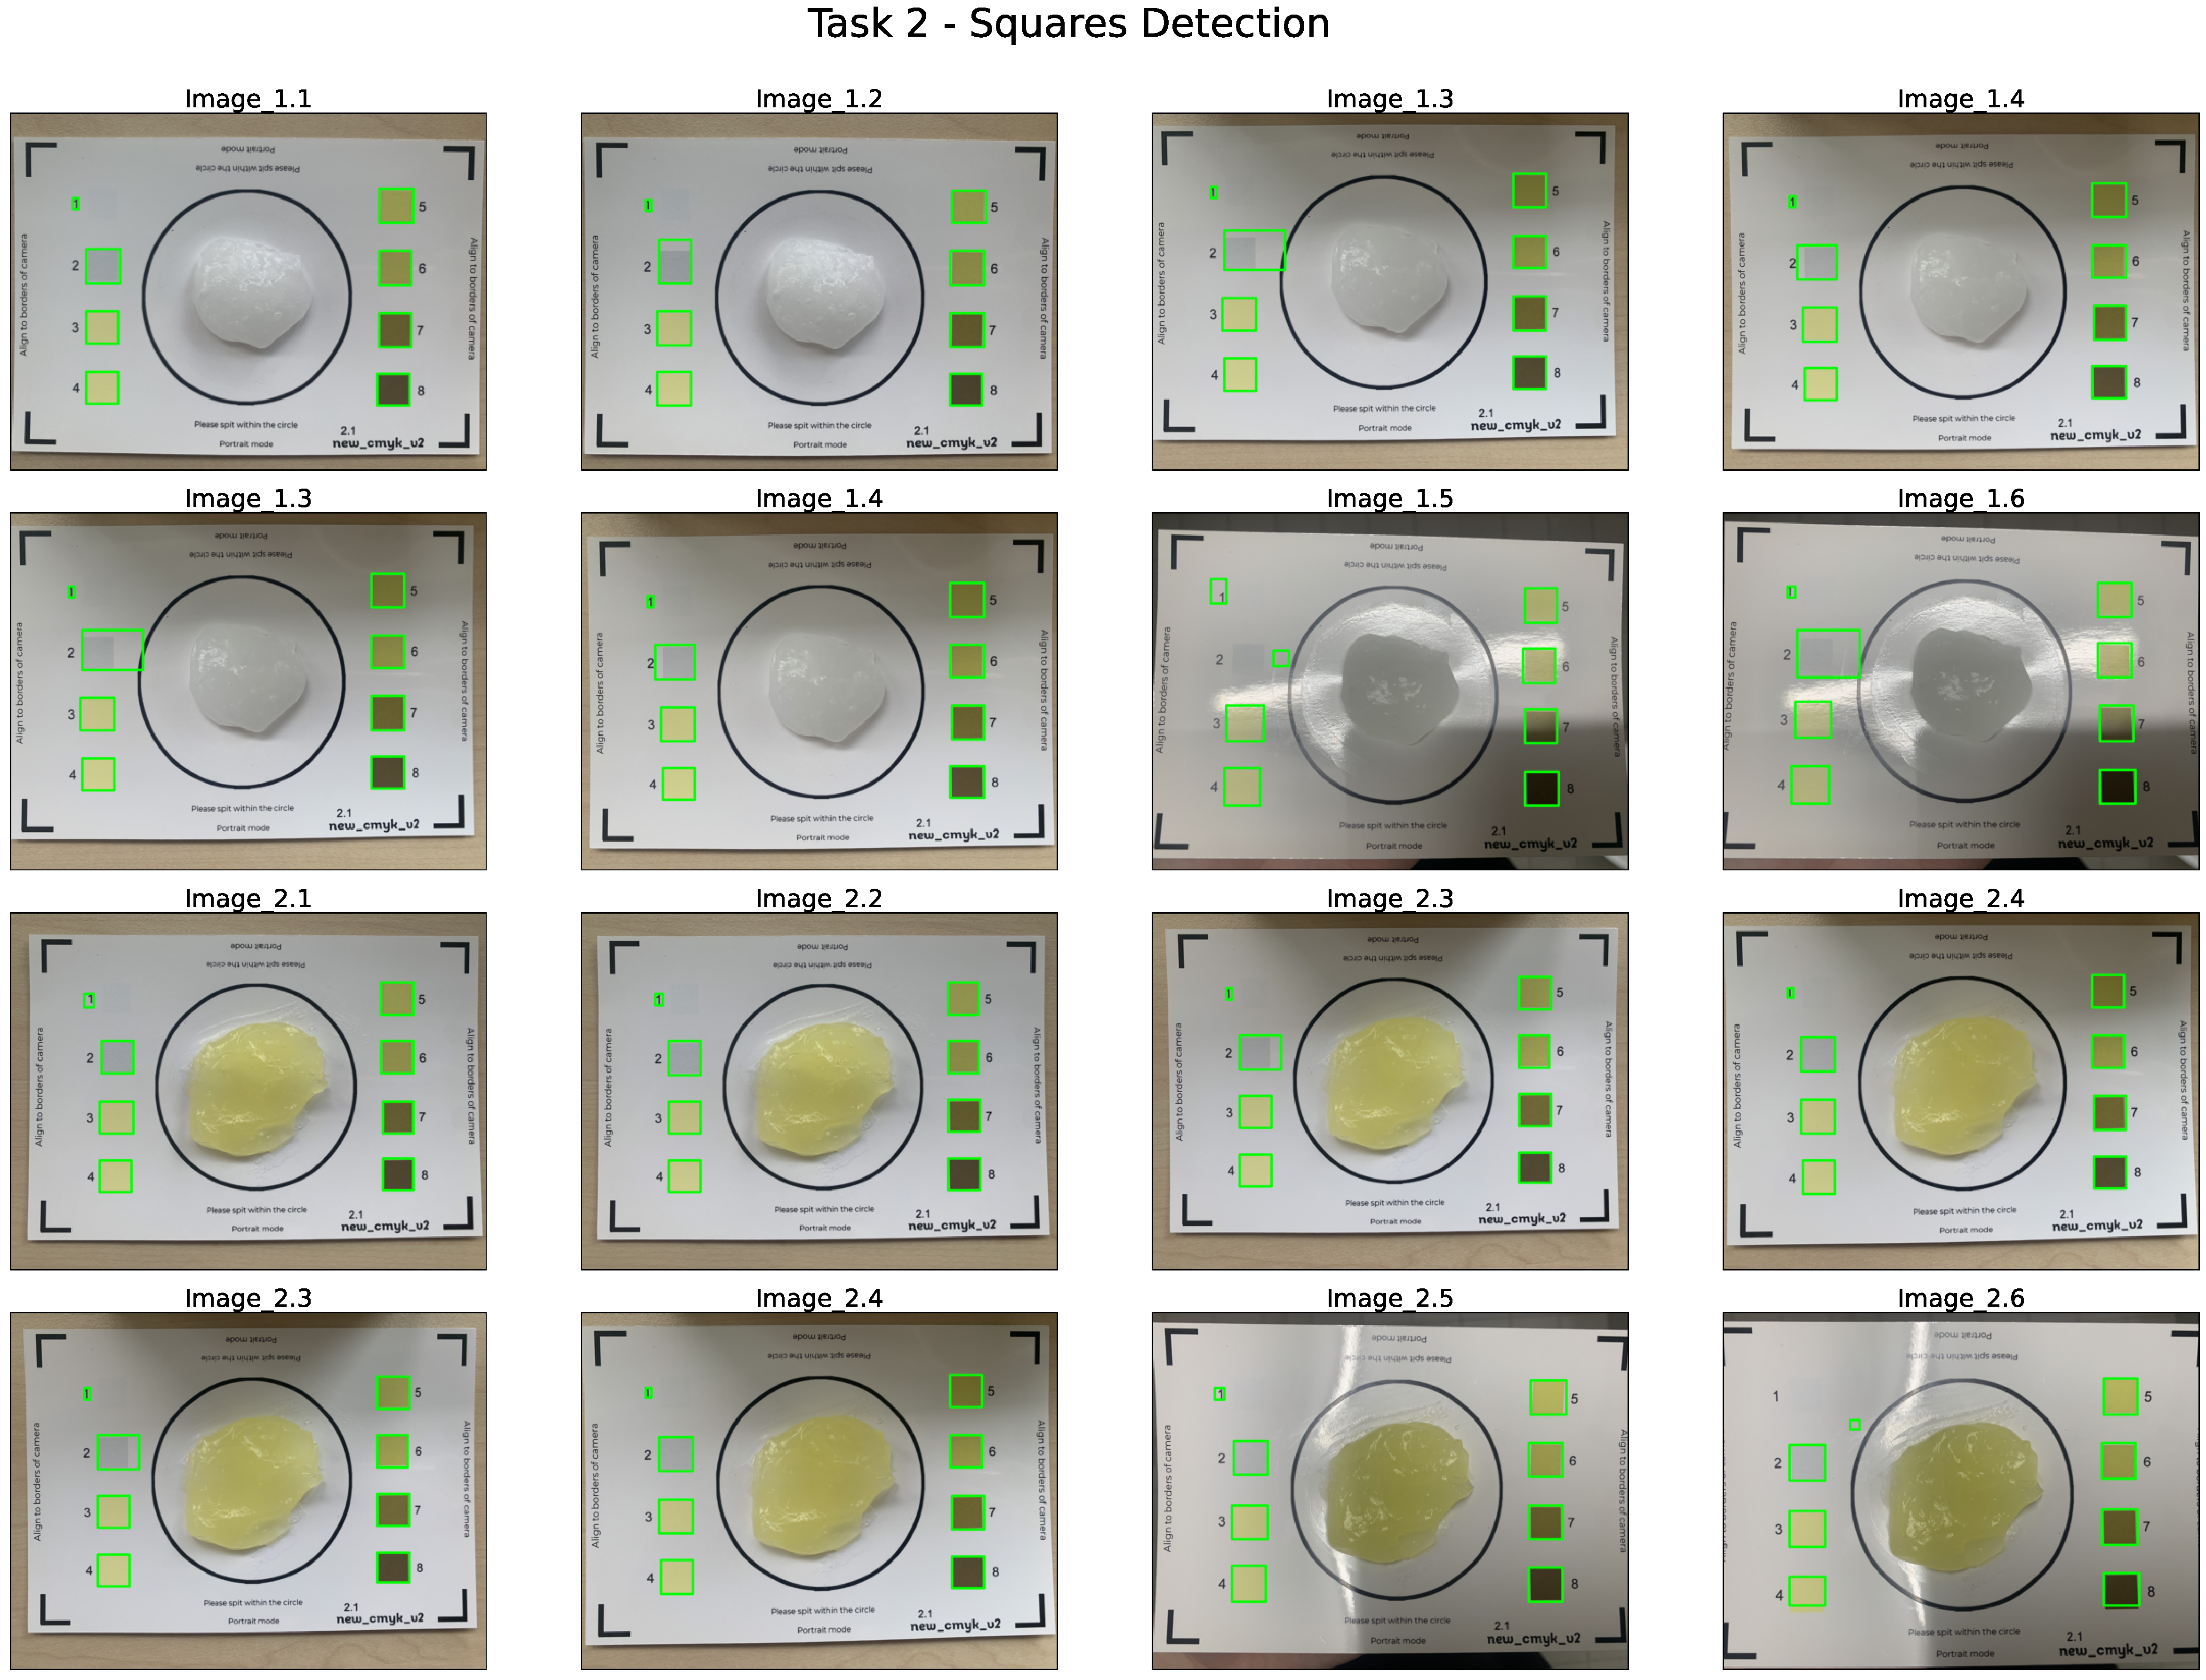
\includegraphics[width=\textwidth]{figs/task2.pdf}} 
	\caption{All results from Task 2.}
	\label{fig: task2-all}
\end{figure}

\newpage 

\begin{figure}[h]
    \centerline{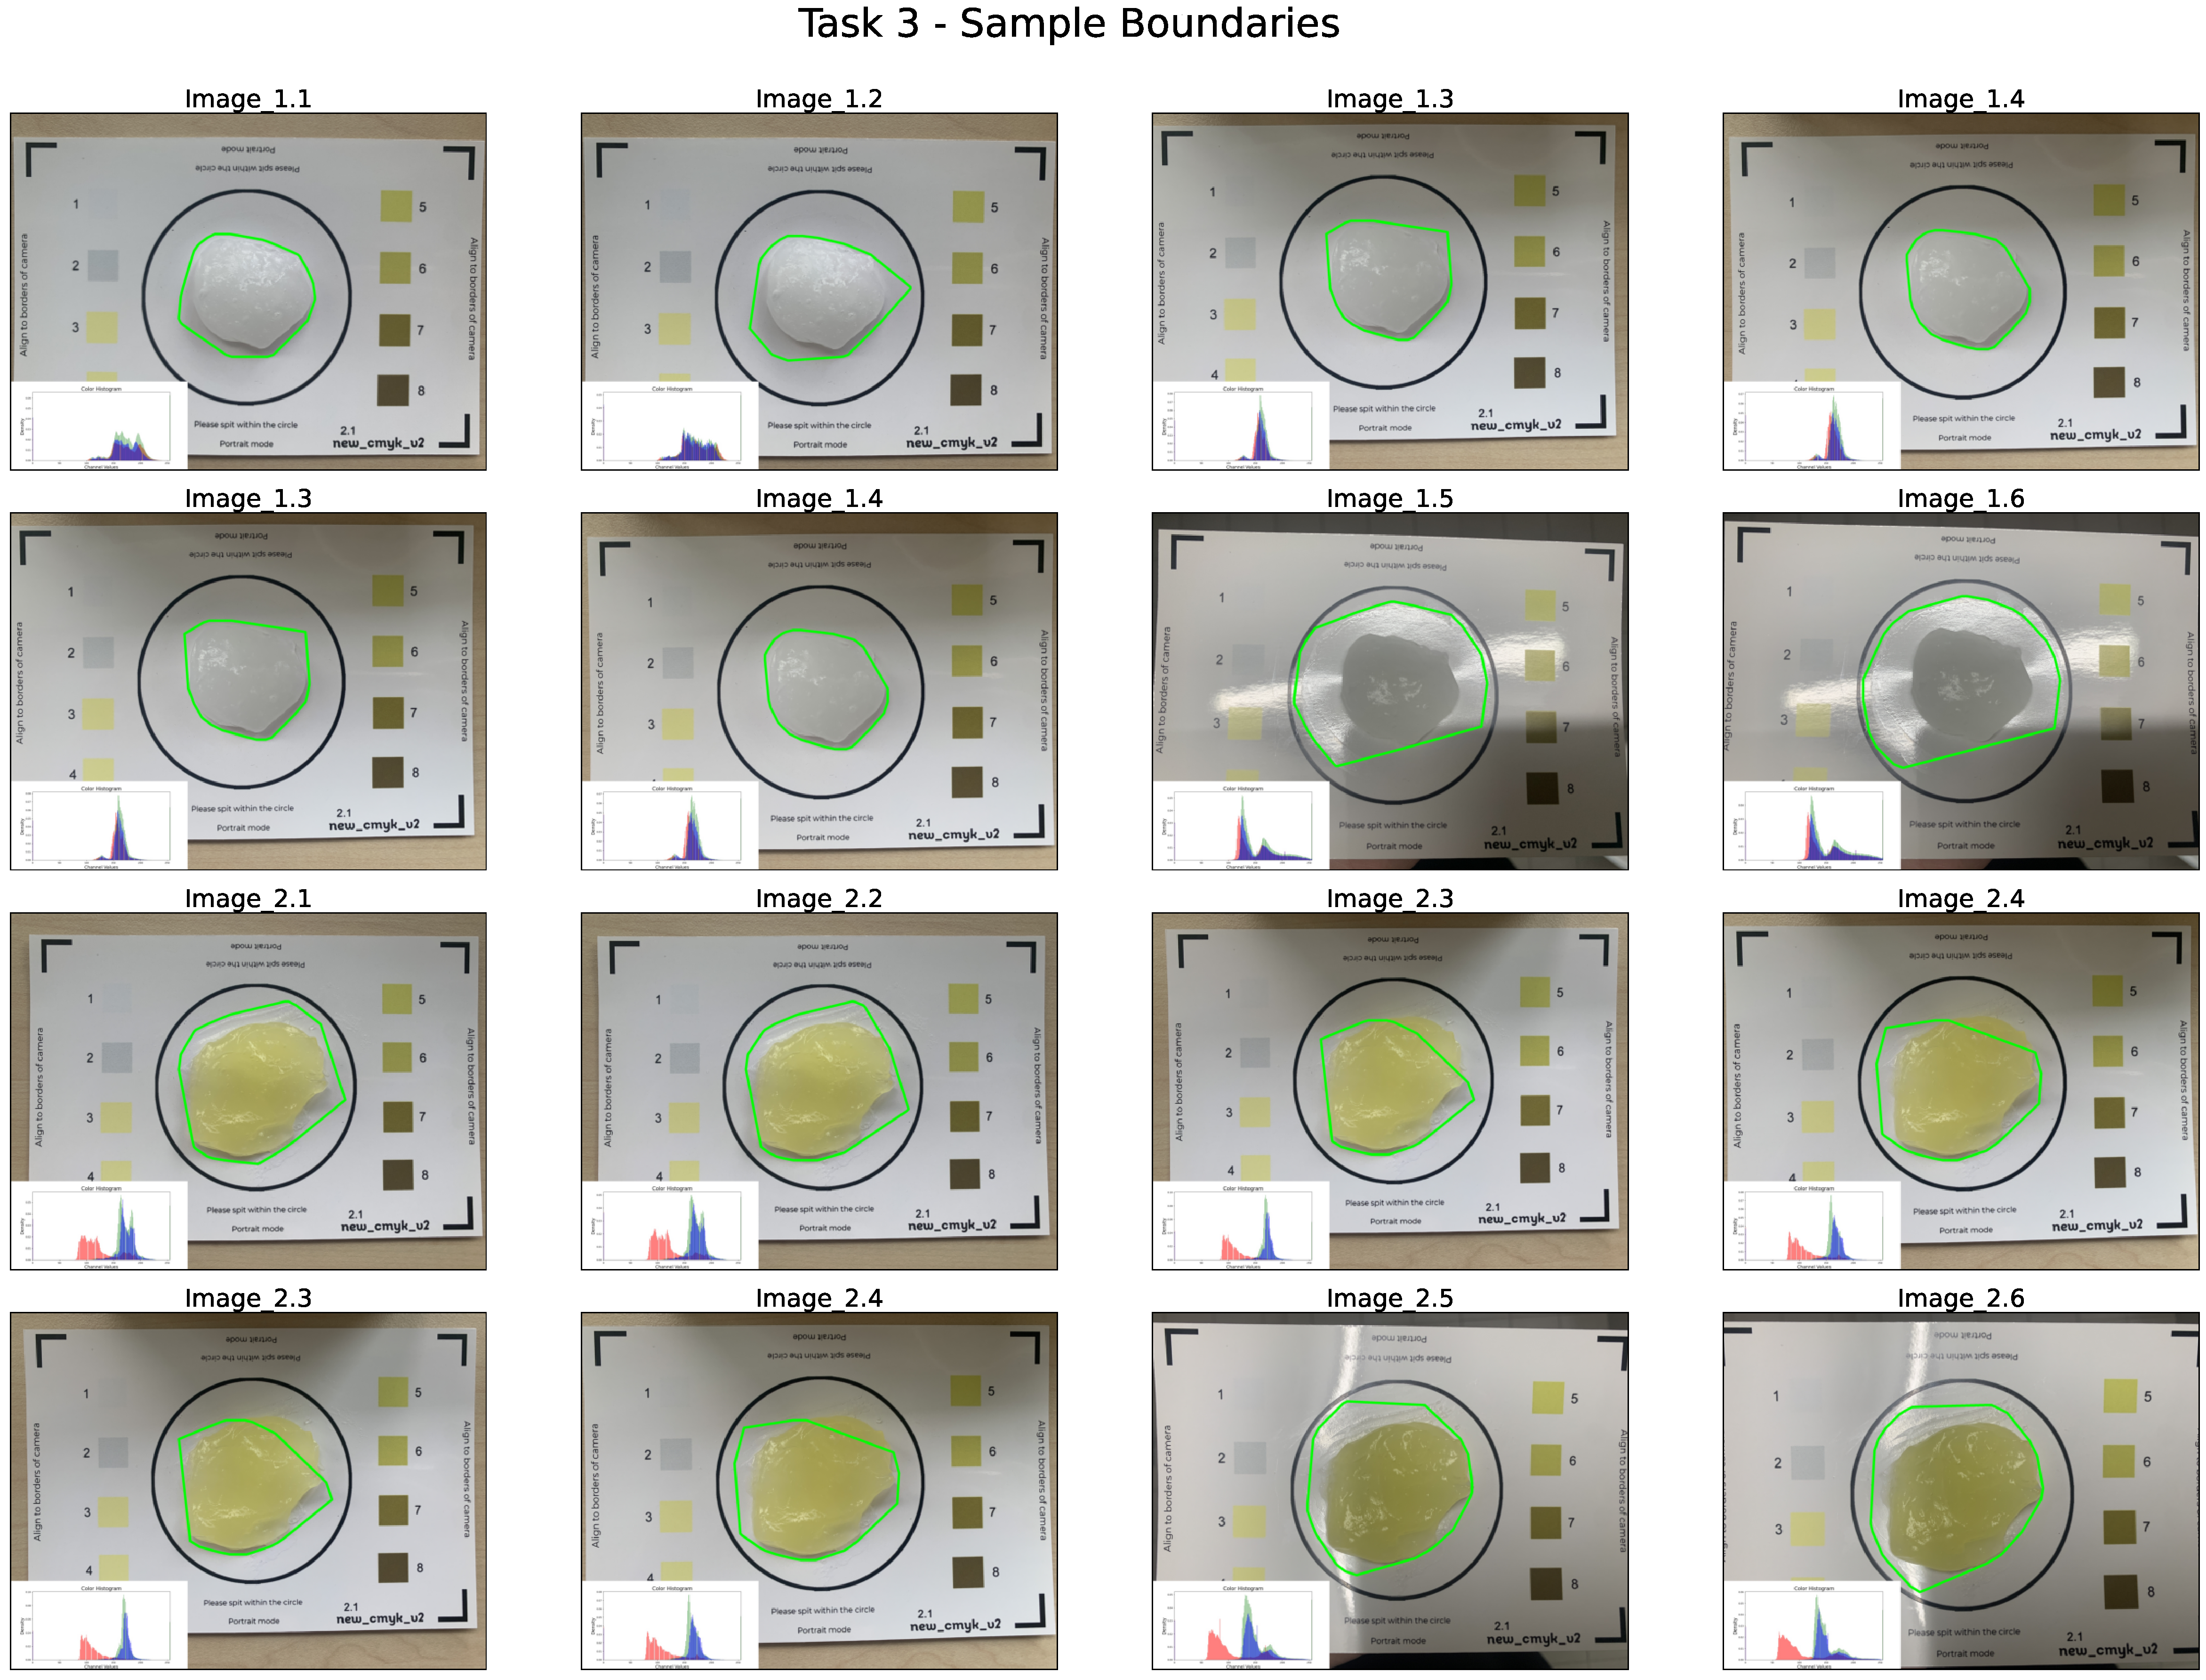
\includegraphics[width=\textwidth]{figs/task3.pdf}} 
	\caption{All results from Task 3.}
	\label{fig: task3-all}
\end{figure}

\newpage 
\begin{figure}[h]
    \centerline{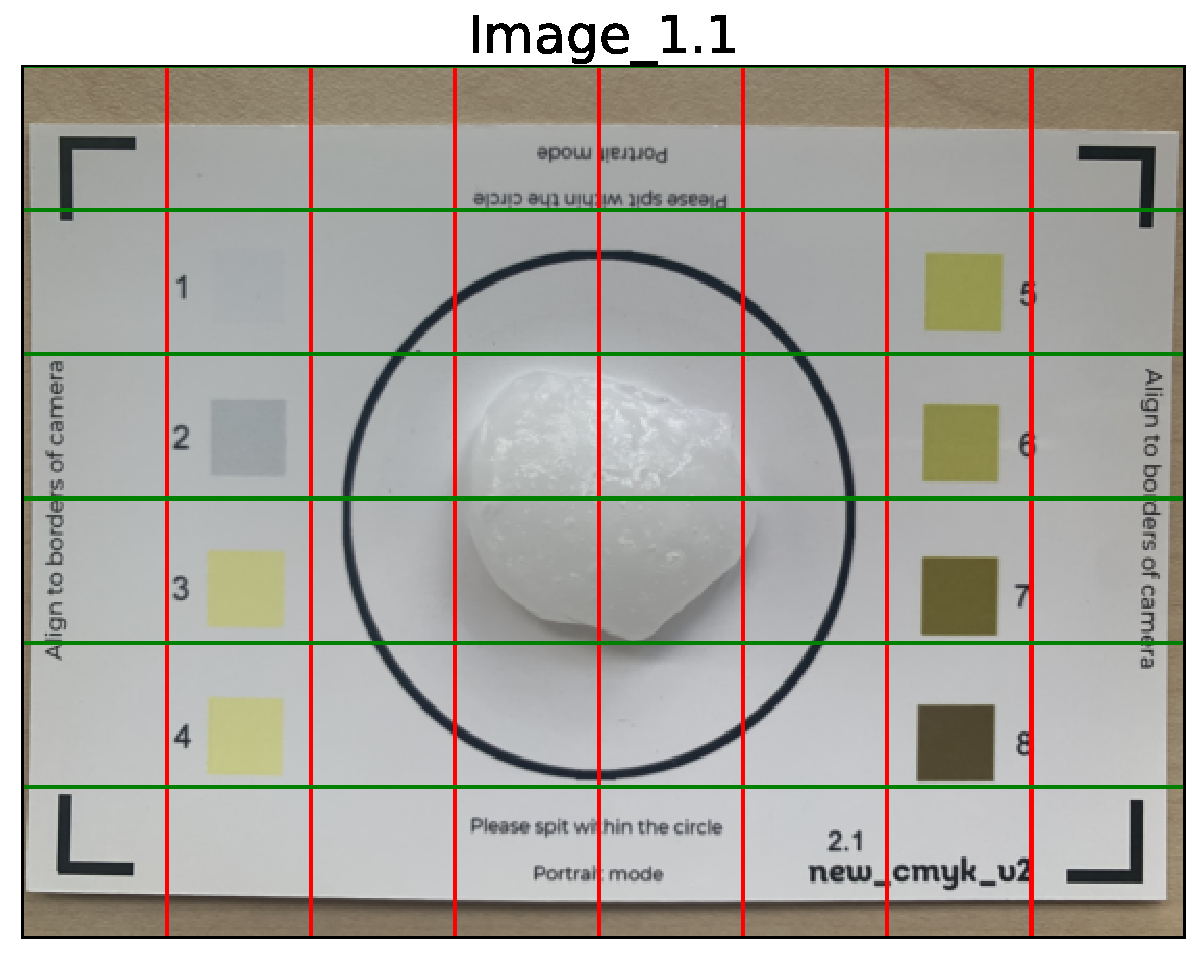
\includegraphics[width=.85\textwidth]{figs/task2-grid.pdf}} 
	\caption{Grid is used to separate the squares, the grid is chose arbitrarily from visual inspection of the samples. This method can be made more robust by standardizing the images' boundaries first.}
	\label{fig: task2-grid}
\end{figure}

\begin{figure}[h]
    \centerline{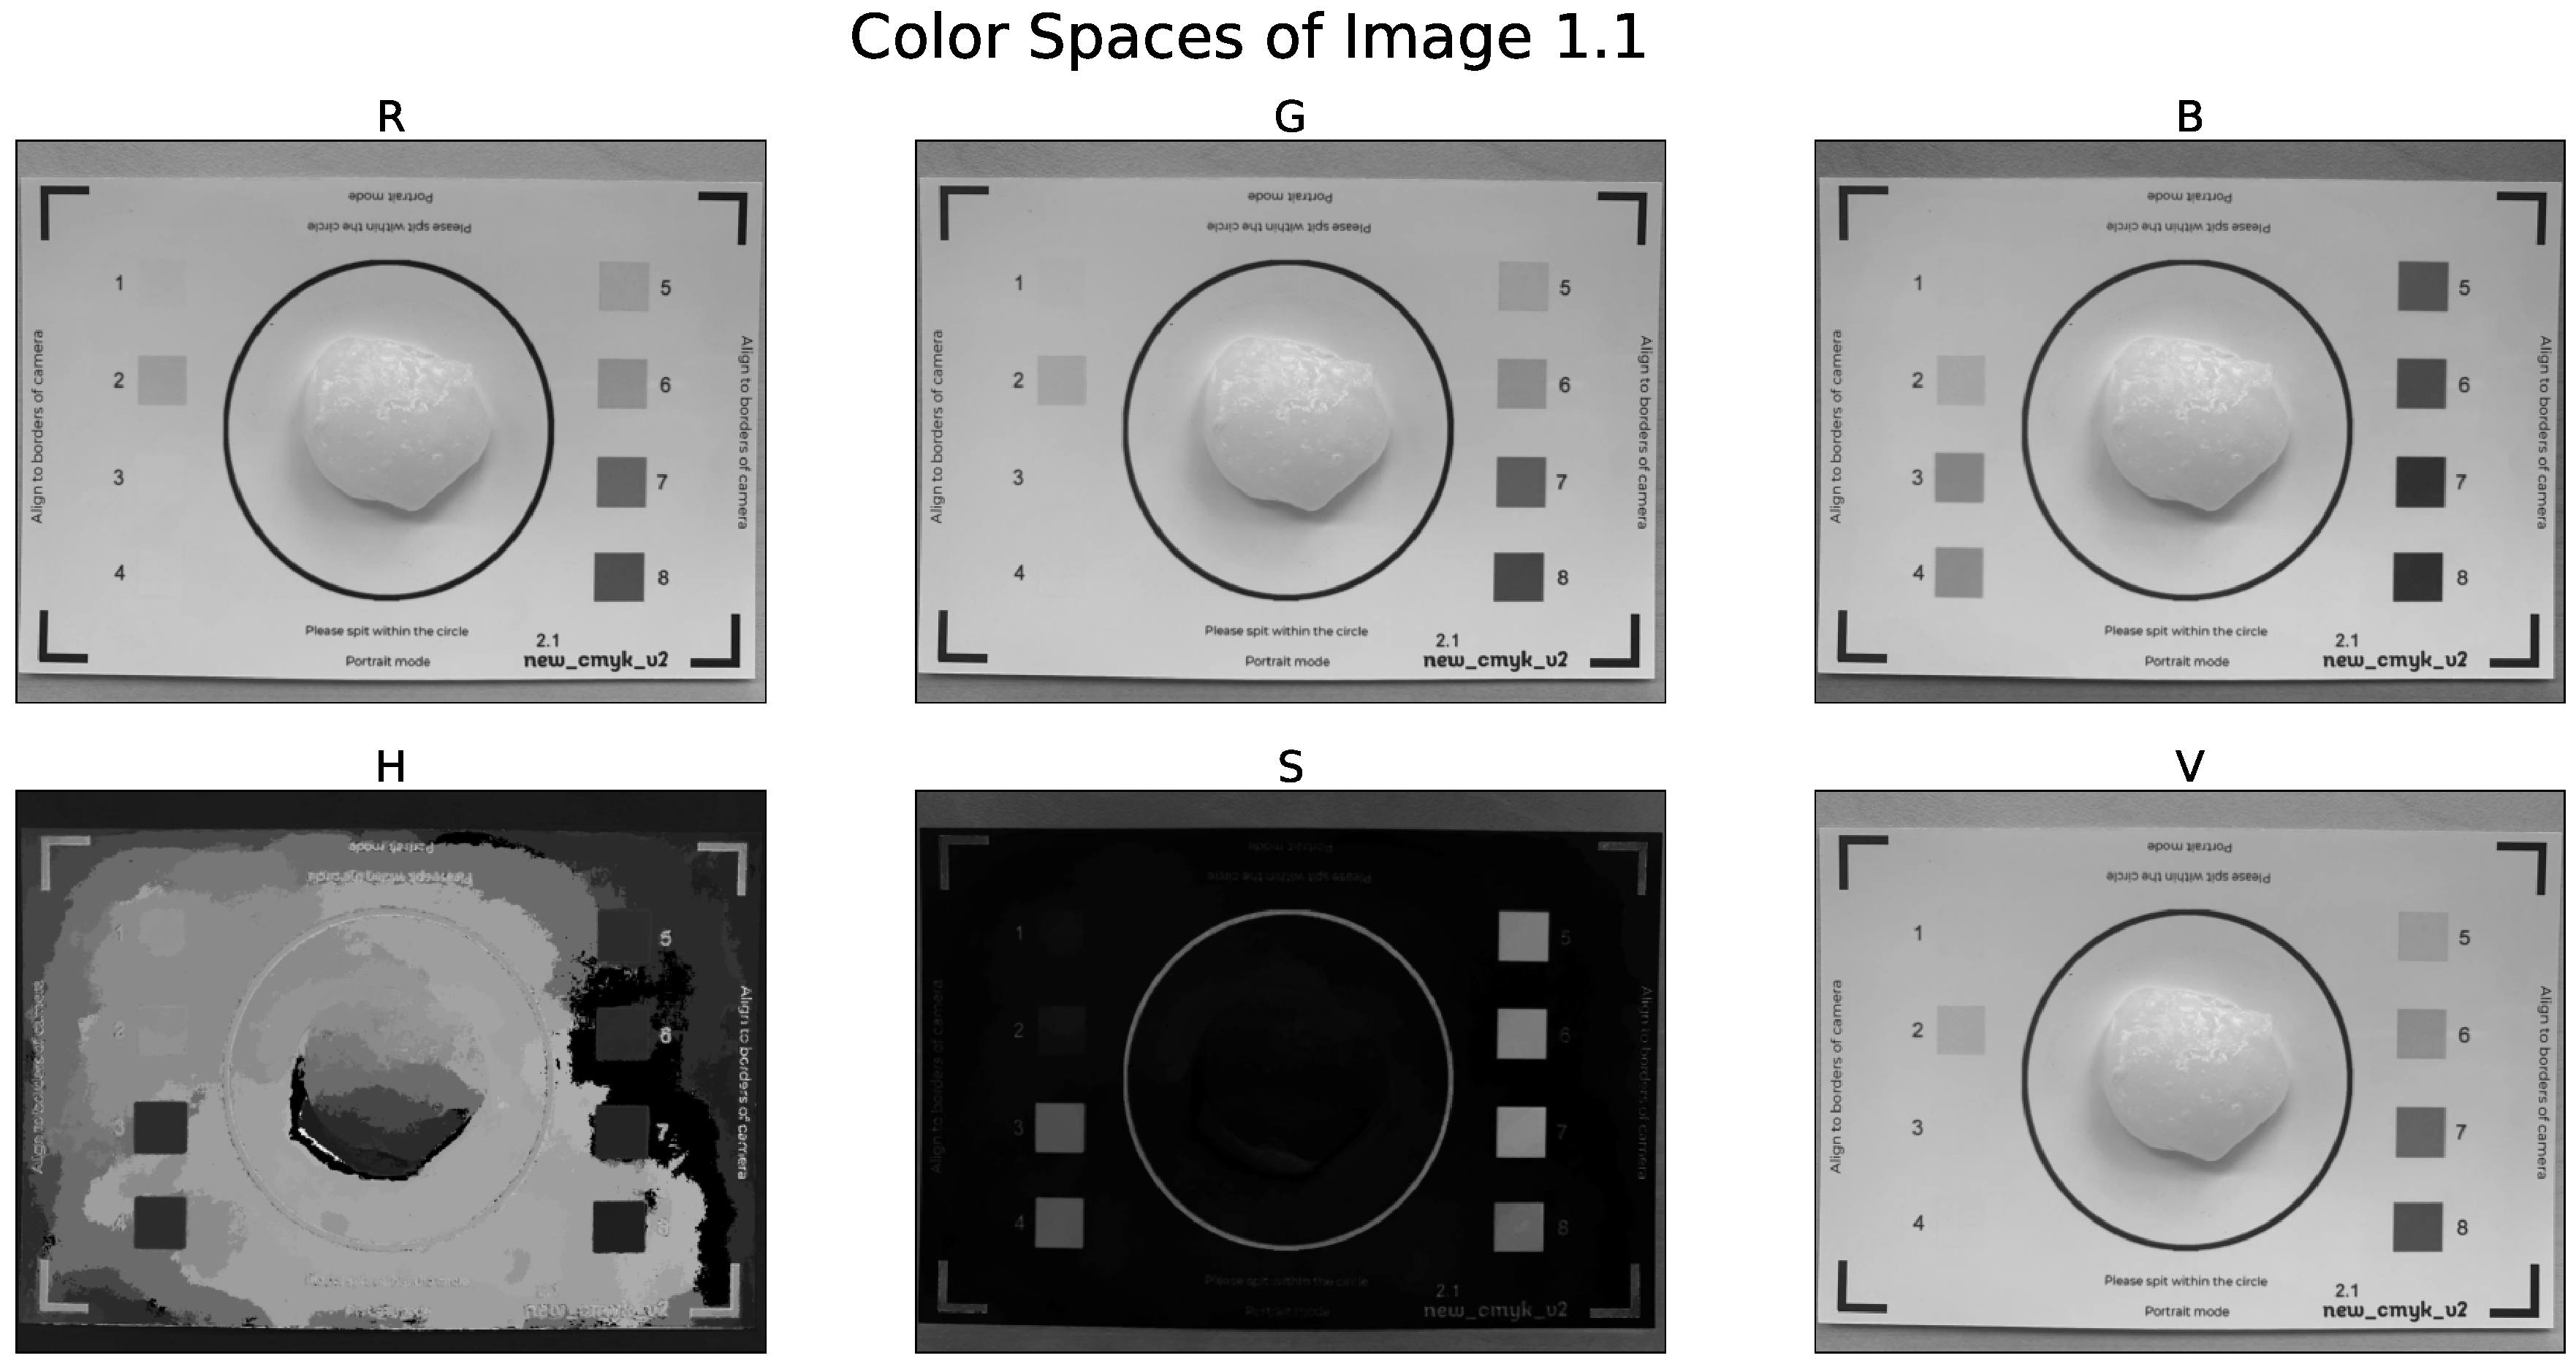
\includegraphics[width=\textwidth]{figs/task2-color.pdf}} 
	\caption{RGB and HSV color spaces of and Image. Notice that for square 2, the blue channel separates the square most from the bacground, while for square 3-8, the S channel separates the square most from the background. No channel clearly separate square 1 with the background.}
	\label{fig: task2-color}
\end{figure}




\end{document}
